% ============================================================================
% AgentK Runtime — Complete Guide
% A Comprehensive Technical, Business, and Strategic Document
% ============================================================================
\documentclass[12pt,a4paper,openany]{report}

% --- Core Packages ---
\usepackage[utf8]{inputenc}
\usepackage[T1]{fontenc}
\usepackage{lmodern}
\usepackage[margin=2.5cm]{geometry}
\usepackage{graphicx}
\usepackage{hyperref}
\usepackage{xcolor}
\usepackage{listings}
\usepackage{longtable}
\usepackage{booktabs}
\usepackage{enumitem}
\usepackage{amsmath,amssymb}
\usepackage{fancyhdr}
\usepackage{titlesec}
\usepackage{tocloft}
\usepackage{float}
\usepackage{caption}
\usepackage{multicol}
\usepackage{tabularx}
\usepackage{colortbl}
\usepackage{tikz}
\usepackage[most]{tcolorbox}

\usetikzlibrary{shapes.geometric, arrows.meta, positioning, fit, calc}

% --- Brand Colors ---
\definecolor{agentk-blue}{HTML}{1e40af}
\definecolor{agentk-green}{HTML}{059669}
\definecolor{agentk-purple}{HTML}{7c3aed}
\definecolor{agentk-orange}{HTML}{ea580c}
\definecolor{agentk-red}{HTML}{dc2626}
\definecolor{agentk-gray}{HTML}{4b5563}
\definecolor{agentk-light}{HTML}{f0f9ff}
\definecolor{agentk-dark}{HTML}{0f172a}
\definecolor{code-bg}{HTML}{f8fafc}
\definecolor{code-border}{HTML}{e2e8f0}

% --- Hyperref Setup ---
\hypersetup{
    colorlinks=true,
    linkcolor=agentk-blue,
    urlcolor=agentk-purple,
    citecolor=agentk-green,
    pdftitle={AgentK Runtime — Complete Guide},
    pdfauthor={AgentK Team},
    pdfsubject={AI Agent Runtime Operator for Kubernetes},
    pdfkeywords={Kubernetes, AI Agents, ZK-SNARK, TEE, Cost Intelligence}
}

% --- Listings Setup ---
\lstdefinestyle{yaml}{
    basicstyle=\ttfamily\small,
    backgroundcolor=\color{code-bg},
    frame=single,
    rulecolor=\color{code-border},
    breaklines=true,
    breakatwhitespace=true,
    showstringspaces=false,
    keywordstyle=\color{agentk-blue}\bfseries,
    stringstyle=\color{agentk-green},
    commentstyle=\color{agentk-gray}\itshape,
    numbers=left,
    numberstyle=\tiny\color{agentk-gray},
    numbersep=8pt,
    tabsize=2,
    morekeywords={apiVersion,kind,metadata,spec,name,namespace,framework,image,
        protocols,type,port,path,replicas,env,value,description,instruction,model,
        tools,subAgents,url,toolServerRef,proofMode,costBudget,costIntelligence,
        governance,lifecycle,strategy,teeProvider,runtimeClassName,enclaveMemoryMB,
        attestationEndpoint,transportType,protocol,optimizationMode,maxMonthlyCostUSD,
        downgradeModel,costPerTokenUSD,autonomyLevel,policyRefs,toolSandboxRef,
        propagatedHeaders,interactionType,entryPointAgents,owner,tags}
}

\lstdefinestyle{golang}{
    basicstyle=\ttfamily\small,
    backgroundcolor=\color{code-bg},
    frame=single,
    rulecolor=\color{code-border},
    breaklines=true,
    showstringspaces=false,
    keywordstyle=\color{agentk-blue}\bfseries,
    stringstyle=\color{agentk-green},
    commentstyle=\color{agentk-gray}\itshape,
    numbers=left,
    numberstyle=\tiny\color{agentk-gray},
    numbersep=8pt,
    language=Go,
    morekeywords={func,type,struct,interface,return,error,nil,var,const,package,import}
}

\lstdefinestyle{bash}{
    basicstyle=\ttfamily\small,
    backgroundcolor=\color{code-bg},
    frame=single,
    rulecolor=\color{code-border},
    breaklines=true,
    showstringspaces=false,
    keywordstyle=\color{agentk-blue}\bfseries,
    commentstyle=\color{agentk-gray}\itshape,
    language=bash
}

% --- tcolorbox Styles ---
\newtcolorbox{keyconceptbox}[1][]{
    colback=agentk-light,
    colframe=agentk-blue,
    fonttitle=\bfseries,
    title=Key Concept,
    #1
}

\newtcolorbox{analogybox}[1][]{
    colback=green!5!white,
    colframe=agentk-green,
    fonttitle=\bfseries,
    title=Simple Analogy,
    #1
}

\newtcolorbox{warningbox}[1][]{
    colback=red!5!white,
    colframe=agentk-red,
    fonttitle=\bfseries,
    title=Important,
    #1
}

\newtcolorbox{tipbox}[1][]{
    colback=purple!5!white,
    colframe=agentk-purple,
    fonttitle=\bfseries,
    title=Pro Tip,
    #1
}

\newtcolorbox{moneybox}[1][]{
    colback=orange!5!white,
    colframe=agentk-orange,
    fonttitle=\bfseries,
    title=Business Insight,
    #1
}

% --- Header/Footer ---
\pagestyle{fancy}
\fancyhf{}
\fancyhead[L]{\small\textcolor{agentk-gray}{AgentK Runtime — Complete Guide}}
\fancyhead[R]{\small\textcolor{agentk-gray}{\leftmark}}
\fancyfoot[C]{\thepage}
\renewcommand{\headrulewidth}{0.4pt}
\renewcommand{\footrulewidth}{0pt}

% --- Chapter/Section Styling ---
\titleformat{\chapter}[display]
    {\normalfont\huge\bfseries\color{agentk-blue}}
    {\chaptertitlename\ \thechapter}{20pt}{\Huge}
\titleformat{\section}
    {\normalfont\Large\bfseries\color{agentk-blue}}
    {\thesection}{1em}{}
\titleformat{\subsection}
    {\normalfont\large\bfseries\color{agentk-purple}}
    {\thesubsection}{1em}{}

% --- Document Start ---
\begin{document}

% ============================================================================
% TITLE PAGE
% ============================================================================
\begin{titlepage}
\centering
\vspace*{2cm}

{\Huge\bfseries\textcolor{agentk-blue}{AgentK Runtime}\par}
\vspace{0.5cm}
{\LARGE\textcolor{agentk-purple}{Complete Guide}\par}
\vspace{1cm}
{\Large\textcolor{agentk-gray}{The Kubernetes-Native Operating System for AI Agents}\par}

\vspace{2cm}

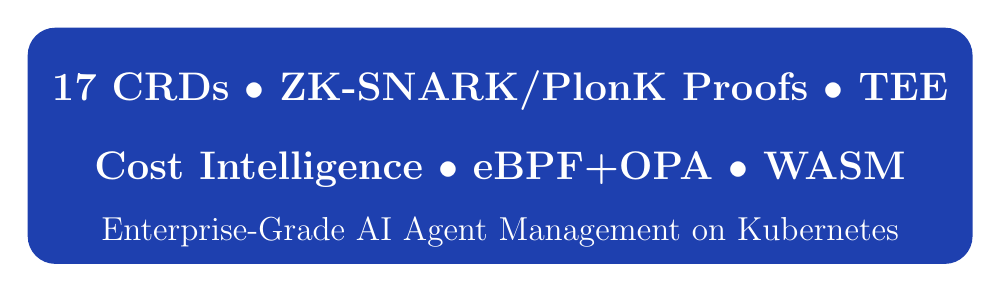
\begin{tikzpicture}
    \fill[agentk-blue, rounded corners=10pt] (0,0) rectangle (12,3);
    \node[white, font=\Large\bfseries] at (6,2.2) {17 CRDs $\bullet$ ZK-SNARK/PlonK Proofs $\bullet$ TEE};
    \node[white, font=\Large\bfseries] at (6,1.2) {Cost Intelligence $\bullet$ eBPF+OPA $\bullet$ WASM};
    \node[white, font=\large] at (6,0.4) {Enterprise-Grade AI Agent Management on Kubernetes};
\end{tikzpicture}

\vspace{2cm}

{\large
\textbf{Product Features} $\bullet$ \textbf{Competitive Analysis} $\bullet$ \textbf{Business Strategy}\\[0.3cm]
\textbf{Technical Deep-Dive} $\bullet$ \textbf{Launch Roadmap} $\bullet$ \textbf{Funding Guide}
}

\vspace{2cm}

{\large\textcolor{agentk-gray}{Version 1.0 — March 2026}\par}
\vspace{0.5cm}
{\normalsize\textcolor{agentk-gray}{Built with real cryptographic proofs (gnark), real TEE attestation (ECDSA P-256),}\par}
{\normalsize\textcolor{agentk-gray}{real-time cost intelligence, and 30+ Prometheus metrics}\par}

\vfill
{\small\textcolor{agentk-gray}{Apache License 2.0 $\bullet$ github.com/Roncode-enter/Ronak-agentk-runtime}\par}
\end{titlepage}

% ============================================================================
% TABLE OF CONTENTS
% ============================================================================
\tableofcontents
\newpage

% ############################################################################
% PART I: PRODUCT FEATURES
% ############################################################################
\part{Product Features — Explained Simply}

% ============================================================================
% CHAPTER 1: WHAT IS AGENTK?
% ============================================================================
\chapter{What is AgentK?}

\section{The Simplest Explanation}

Imagine you have a school with 100 students (these are your \textbf{AI agents} — programs that can think, talk, and do tasks). Each student needs:

\begin{itemize}
    \item A classroom to sit in (a \textbf{computer/server} to run on)
    \item A teacher watching them (a \textbf{health check} to make sure they're working)
    \item Rules to follow (a \textbf{policy} so they don't do bad things)
    \item A report card (a \textbf{status} showing how well they're doing)
    \item A budget for lunch money (a \textbf{cost limit} so they don't spend too much)
\end{itemize}

Now imagine trying to manage 100 students manually — assigning classrooms, checking if anyone is sick, making sure nobody is breaking rules, tracking budgets. That's impossible for a human to do all day.

\begin{analogybox}
\textbf{AgentK} is like the world's best school principal — it automatically manages all your AI agents. You just tell it ``I want a student named Weather-Bot who can answer weather questions'', and AgentK handles everything else: finding a classroom, monitoring health, enforcing rules, tracking costs, and reporting status.
\end{analogybox}

\section{What is Kubernetes?}

Before we understand AgentK, we need to understand \textbf{Kubernetes} (often called ``K8s'').

\begin{keyconceptbox}
\textbf{Kubernetes} is like a giant building manager for computers. If you have 10 servers (computers), Kubernetes decides which program runs on which server, restarts programs that crash, and balances the workload — all automatically. It's made by Google and used by Netflix, Spotify, Airbnb, and almost every big tech company.
\end{keyconceptbox}

Kubernetes works with \textbf{YAML files} — simple text files where you describe what you want. For example:

\begin{lstlisting}[style=yaml, caption={A simple Kubernetes instruction}]
# "Hey Kubernetes, please run 3 copies of my website"
apiVersion: apps/v1
kind: Deployment
metadata:
  name: my-website
spec:
  replicas: 3
\end{lstlisting}

You write what you \textit{want}, and Kubernetes figures out \textit{how} to make it happen. This is called \textbf{declarative management}.

\section{What is a Kubernetes Operator?}

A \textbf{Kubernetes Operator} is a special program that teaches Kubernetes new tricks.

\begin{analogybox}
Think of Kubernetes as a phone. Out of the box, it can make calls and send texts. But when you install apps (like Instagram or Uber), your phone learns new abilities. A Kubernetes Operator is like an app for Kubernetes — it teaches Kubernetes how to manage a new type of thing (in our case, AI agents).
\end{analogybox}

AgentK is a \textbf{Kubernetes Operator} that teaches Kubernetes how to manage AI agents. After you install AgentK, Kubernetes suddenly understands commands like:

\begin{lstlisting}[style=yaml, caption={Creating an AI agent with AgentK}]
apiVersion: runtime.agentic-layer.ai/v1alpha1
kind: Agent
metadata:
  name: my-weather-bot
spec:
  framework: google-adk
  description: "A weather information agent"
  instruction: "Help users check the weather"
  model: "gemini/gemini-2.5-flash"
  protocols:
    - type: A2A
  replicas: 2
\end{lstlisting}

\section{The 17 Custom Resource Definitions (CRDs)}

AgentK adds \textbf{17 new types of objects} that Kubernetes can manage. Think of these as 17 new app features:

\begin{longtable}{p{4cm}p{8cm}p{2cm}}
\toprule
\textbf{CRD Name} & \textbf{What It Does (Simple)} & \textbf{Category} \\
\midrule
\endhead
Agent & Deploys and manages an AI agent & Core \\
ToolServer & Runs external tools that agents can use & Core \\
AgenticWorkforce & Groups agents into teams & Core \\
\midrule
AgentGateway & Front door for accessing agents & Gateway \\
AgentGatewayClass & Type of front door (KrakenD, Envoy) & Gateway \\
AIGateway & Routes requests to AI models & Gateway \\
AIGatewayClass & Type of AI model router & Gateway \\
ToolGateway & Routes requests to tool servers & Gateway \\
ToolGatewayClass & Type of tool router & Gateway \\
\midrule
Guard & Safety filter for AI responses & Security \\
GuardrailProvider & External safety service connection & Security \\
Policy & Network/system rules (eBPF + OPA) & Security \\
ToolSandbox & Secure box for running tools (WASM) & Security \\
ConfidentialAgent & Agent running in sealed hardware (TEE) & Security \\
\midrule
Swarm & Coordinates multiple agents together & Advanced \\
SimulationPreview & Dry-run before deploying & Advanced \\
AgentRuntimeConfig & Cluster-wide default settings & Config \\
\bottomrule
\caption{All 17 Custom Resource Definitions in AgentK}
\end{longtable}

\section{The 5 Moats — What Makes AgentK Special}

A ``moat'' in business means a feature that's so hard to copy that competitors can't easily replicate it. AgentK has \textbf{5 moats}:

\begin{enumerate}[label=\textbf{Moat \arabic*:}]
    \item \textbf{WASM Sandbox} — Run tools in a sealed container (like a quarantine room)
    \item \textbf{eBPF + OPA Policies} — Control network access at the Linux kernel level
    \item \textbf{Merkle Verification} — Tamper-proof audit trail using SHA-256 hash chains
    \item \textbf{Predictive Cost Intelligence} — Real-time cost monitoring with auto-downgrade
    \item \textbf{Swarm Coordination} — 4 strategies for multi-agent teamwork
\end{enumerate}

Plus \textbf{3 Sovereign features} (premium):
\begin{enumerate}[label=\textbf{Sovereign \arabic*:}]
    \item \textbf{ZK-SNARK/PlonK Proofs} — Mathematical proof that computation was correct
    \item \textbf{TEE Attestation} — Hardware-sealed execution with cryptographic verification
    \item \textbf{Governance Tiers} — Autonomy levels 1–5 with human-in-the-loop approval
\end{enumerate}


% ============================================================================
% CHAPTER 2: CORE CRDs
% ============================================================================
\chapter{Core CRDs — Agent, ToolServer, Workforce}

\section{The Agent CRD — Your AI Worker}

The \textbf{Agent} is the most important resource. It represents a single AI agent — a program that can think, respond to questions, use tools, and talk to other agents.

\begin{keyconceptbox}
When you create an \texttt{Agent} resource in Kubernetes, AgentK automatically:
\begin{enumerate}
    \item Creates a \textbf{Deployment} (the running program)
    \item Creates a \textbf{Service} (a network address so others can talk to it)
    \item Sets up \textbf{health checks} (so Kubernetes knows if it's alive)
    \item Tracks \textbf{status} (ready/not ready, cost, proof chain)
\end{enumerate}
\end{keyconceptbox}

\subsection{Template-Based Agents (Easy Mode)}

The easiest way to create an agent — just describe what you want:

\begin{lstlisting}[style=yaml, caption={A template-based agent}]
apiVersion: runtime.agentic-layer.ai/v1alpha1
kind: Agent
metadata:
  name: news-agent
spec:
  framework: google-adk
  description: "A news agent that fetches articles"
  instruction: "You are a news agent. Fetch and summarize articles."
  model: "gemini/gemini-2.5-flash"
  tools:
    - name: news_fetcher
      toolServerRef:
        name: news-fetcher-toolserver
  protocols:
    - type: A2A
  replicas: 2
  env:
    - name: GEMINI_API_KEY
      value: "your-api-key-here"
\end{lstlisting}

\subsection{Custom Image Agents (Full Control)}

When you need specific libraries or frameworks:

\begin{lstlisting}[style=yaml, caption={A custom image agent}]
apiVersion: runtime.agentic-layer.ai/v1alpha1
kind: Agent
metadata:
  name: weather-agent
spec:
  framework: google-adk
  image: ghcr.io/agentic-layer/weather-agent:0.3.0
  protocols:
    - type: A2A
  replicas: 1
\end{lstlisting}

\subsection{Agent Configuration Options}

\begin{longtable}{p{4cm}p{8cm}p{2.5cm}}
\toprule
\textbf{Field} & \textbf{What It Does} & \textbf{Required?} \\
\midrule
\endhead
\texttt{framework} & Which AI framework to use (google-adk, msaf, custom) & Yes \\
\texttt{image} & Custom Docker image for the agent & No \\
\texttt{description} & What the agent does (shown to users) & No \\
\texttt{instruction} & System prompt that guides the agent's behavior & No \\
\texttt{model} & AI model to use (e.g., gemini-2.5-flash) & No \\
\texttt{protocols} & Communication protocols (A2A) & Yes \\
\texttt{replicas} & How many copies to run & No (default: 1) \\
\texttt{tools} & External tools the agent can use & No \\
\texttt{subAgents} & Other agents this agent can delegate to & No \\
\texttt{env} & Environment variables & No \\
\texttt{resources} & CPU/memory limits & No \\
\texttt{proofMode} & ZK proof type (merkle-only, snark-groth16, plonk-universal) & No \\
\texttt{costBudget} & Monthly spending limit & No \\
\texttt{costIntelligence} & Real-time cost optimization settings & No \\
\texttt{governance} & Autonomy level (1–5) & No \\
\texttt{lifecycle} & Deployment strategy (rolling, canary, blue-green) & No \\
\texttt{policyRefs} & Security policies to enforce & No \\
\texttt{toolSandboxRef} & WASM sandbox for secure tool execution & No \\
\bottomrule
\caption{Agent spec fields}
\end{longtable}

\section{The ToolServer CRD — External Tools}

A \textbf{ToolServer} is a separate service that provides tools for agents to use.

\begin{analogybox}
If an agent is a student, a ToolServer is like a calculator or a dictionary that the student can borrow. The student (agent) asks the tool for help, gets the answer, and continues working.
\end{analogybox}

\begin{lstlisting}[style=yaml, caption={A ToolServer for code documentation}]
apiVersion: runtime.agentic-layer.ai/v1alpha1
kind: ToolServer
metadata:
  name: context7-toolserver
spec:
  protocol: mcp
  transportType: http
  image: mcp/context7:latest
  port: 8080
  replicas: 2
\end{lstlisting}

ToolServers use the \textbf{Model Context Protocol (MCP)} — a standard way for AI agents to talk to tools. It supports two transport types:
\begin{itemize}
    \item \texttt{http} — Standard HTTP requests (most common)
    \item \texttt{sse} — Server-Sent Events (for streaming responses)
\end{itemize}

\section{The AgenticWorkforce CRD — Team of Agents}

An \textbf{AgenticWorkforce} groups multiple agents into a team with automatic discovery of all connected agents and tools.

\begin{lstlisting}[style=yaml, caption={An agentic workforce}]
apiVersion: runtime.agentic-layer.ai/v1alpha1
kind: AgenticWorkforce
metadata:
  name: customer-service-team
spec:
  name: "Customer Service Team"
  description: "Handles customer inquiries"
  owner: "platform-team@company.com"
  tags:
    - customer-service
    - production
  entryPointAgents:
    - name: main-support-agent
    - name: billing-agent
\end{lstlisting}

\begin{keyconceptbox}
\textbf{Transitive Discovery}: When you create a workforce with 2 entry-point agents, AgentK automatically discovers ALL sub-agents and tools that those agents use — even sub-agents of sub-agents. This gives you complete visibility into your entire agent ecosystem.
\end{keyconceptbox}


% ============================================================================
% CHAPTER 3: GATEWAYS
% ============================================================================
\chapter{Gateways — The Front Door}

\section{What is a Gateway?}

\begin{analogybox}
A gateway is like the reception desk at a hotel. Instead of visitors going directly to hotel rooms (agents), they first check in at the reception (gateway), which directs them to the right room. This provides security, load balancing, and a single entry point.
\end{analogybox}

\section{AgentGateway}

The \textbf{AgentGateway} provides a unified access point for all your agents:

\begin{lstlisting}[style=yaml, caption={An AgentGateway}]
apiVersion: runtime.agentic-layer.ai/v1alpha1
kind: AgentGateway
metadata:
  name: agent-gateway
spec:
  replicas: 1
  timeout: 5m0s
\end{lstlisting}

It supports multiple implementations (called ``classes''):
\begin{itemize}
    \item \textbf{KrakenD} — High-performance API gateway
    \item \textbf{Envoy} — Cloud-native proxy
    \item \textbf{Nginx} — Traditional web server proxy
\end{itemize}

\section{AIGateway}

The \textbf{AIGateway} routes requests to different AI models. It includes:
\begin{itemize}
    \item \textbf{AI Model definitions} — which models are available (name + provider)
    \item \textbf{Guardrail integration} — safety filters on AI responses
    \item \textbf{Port configuration} — where to listen (default: 80)
\end{itemize}

\section{ToolGateway}

The \textbf{ToolGateway} routes requests to tool servers, providing:
\begin{itemize}
    \item Centralized access to all tools
    \item Load balancing across tool server replicas
    \item Health checking of tool servers
\end{itemize}


% ============================================================================
% CHAPTER 4: GUARDRAILS
% ============================================================================
\chapter{Guardrails — Safety Filters}

\section{Why Guardrails?}

AI agents can sometimes generate harmful, biased, or inappropriate content. \textbf{Guardrails} are safety filters that check AI responses before they reach the user.

\begin{analogybox}
Think of guardrails like a spell-checker and content filter combined. Before an AI agent's response goes to the user, it passes through a safety check: ``Is this response appropriate? Does it contain personal information? Is it harmful?'' If it fails the check, the response is blocked or modified.
\end{analogybox}

\section{Guard CRD}

A \textbf{Guard} defines when and how to check responses:

\begin{itemize}
    \item \texttt{pre\_call} — Check the user's input BEFORE the AI processes it
    \item \texttt{post\_call} — Check the AI's response BEFORE sending to the user
    \item \texttt{during\_call} — Monitor the conversation in real-time
\end{itemize}

\section{GuardrailProvider CRD}

A \textbf{GuardrailProvider} connects to an external safety service:

\begin{longtable}{p{4cm}p{9cm}}
\toprule
\textbf{Provider} & \textbf{What It Does} \\
\midrule
OpenAI Moderation & Uses OpenAI's content moderation API \\
Amazon Bedrock & Uses AWS Bedrock guardrails \\
Presidio & Microsoft's PII (Personal Identifiable Information) detection \\
\bottomrule
\caption{Supported guardrail providers}
\end{longtable}


% ============================================================================
% CHAPTER 5: ZERO-KNOWLEDGE PROOFS
% ============================================================================
\chapter{Zero-Knowledge Proofs — Proving Without Revealing}

\section{What is a Zero-Knowledge Proof?}

This is one of the most mind-bending concepts in computer science, but let's make it simple.

\begin{analogybox}
\textbf{The Color-Blind Friend Puzzle}

Imagine your friend is color-blind and you have two balls — one red and one green. Your friend thinks they're the same color. You want to PROVE they're different WITHOUT telling your friend which one is red and which is green.

Here's how: Your friend holds one ball in each hand, then puts them behind their back. They either swap or don't swap (randomly), then show you both balls again. You can always tell whether they swapped because YOU can see the colors. After doing this 100 times, your friend is convinced the balls are different — but they STILL don't know which is red and which is green.

That's a zero-knowledge proof: you proved something is true without revealing any secret information.
\end{analogybox}

\section{Why Do AI Agents Need ZK Proofs?}

When an AI agent makes a decision (like approving a loan or diagnosing a disease), you want to be able to PROVE:
\begin{enumerate}
    \item The agent actually ran the correct computation
    \item Nobody tampered with the result
    \item The proof chain is intact (no steps were skipped)
\end{enumerate}

Without revealing:
\begin{enumerate}
    \item The agent's internal parameters
    \item The user's private data
    \item The model's proprietary weights
\end{enumerate}

\section{How AgentK's Proof System Works}

AgentK offers \textbf{3 proof modes}:

\subsection{Mode 1: Merkle-Only (Free Tier)}

\begin{keyconceptbox}
\textbf{SHA-256 hash chains}: Each step of the agent's execution is hashed. The hash of step N includes the hash of step N-1, creating an unbreakable chain. If anyone changes one step, all subsequent hashes break.

This is like a paper chain where each link is glued to the previous one — you can't remove a link without breaking the chain.
\end{keyconceptbox}

Formula: $\text{Hash}_n = \text{SHA256}(\text{Hash}_{n-1} \| \text{StepData}_n)$

\subsection{Mode 2: SNARK-Groth16 (Standard Tier)}

This is a \textbf{real zero-knowledge proof} using the Groth16 protocol and the gnark cryptographic library.

\begin{keyconceptbox}
\textbf{The Math Behind It (Simplified)}

AgentK defines a ``circuit'' — a mathematical equation:

$$\text{MiMC}(\text{previousProof} \| \text{secretInput} \| \text{stepIndex}) = \text{expectedOutput}$$

Where:
\begin{itemize}
    \item $\text{previousProof}$ — the proof from the last step (public — everyone sees this)
    \item $\text{stepIndex}$ — which step number we're on (public)
    \item $\text{expectedOutput}$ — what the result should be (public)
    \item $\text{secretInput}$ — the agent's private data (SECRET — only the prover knows this)
\end{itemize}

The prover creates a \textbf{128-byte proof} that says: ``I know a secretInput that makes this equation true'' — without revealing the secretInput.
\end{keyconceptbox}

\textbf{MiMC} is a special hash function designed to work efficiently inside ZK circuits (unlike SHA-256, which is very expensive in ZK).

\textbf{Technical details:}
\begin{itemize}
    \item \textbf{Library}: \texttt{github.com/consensys/gnark} v0.12.0
    \item \textbf{Curve}: BN254 (Barreto-Naehrig 254-bit curve)
    \item \textbf{Proof size}: $\sim$128 bytes
    \item \textbf{Verification time}: $\sim$1 millisecond
    \item \textbf{Setup}: One-time trusted setup ceremony (generates proving key + verifying key)
\end{itemize}

\begin{lstlisting}[style=golang, caption={The actual circuit code (internal/verifiable/circuit.go)}]
type ProofChainCircuit struct {
    PreviousProof  frontend.Variable `gnark:",public"`
    StepIndex      frontend.Variable `gnark:",public"`
    ExpectedOutput frontend.Variable `gnark:",public"`
    SecretInput    frontend.Variable // private (ZK part)
}

func (c *ProofChainCircuit) Define(api frontend.API) error {
    h, _ := mimc.NewMiMC(api)
    h.Write(c.PreviousProof)
    h.Write(c.SecretInput)
    h.Write(c.StepIndex)
    result := h.Sum()
    api.AssertIsEqual(result, c.ExpectedOutput)
    return nil
}
\end{lstlisting}

\subsection{Mode 3: PlonK-Universal (Premium Tier)}

PlonK is a more advanced proof system with one huge advantage: \textbf{universal setup}.

\begin{keyconceptbox}
\textbf{Groth16 vs PlonK}

\begin{tabular}{lcc}
\toprule
\textbf{Feature} & \textbf{Groth16} & \textbf{PlonK} \\
\midrule
Setup ceremony & Per-circuit (must redo for changes) & Universal (one-time for ALL circuits) \\
Proof size & $\sim$128 bytes & $\sim$400 bytes \\
Verification time & $\sim$1ms & $\sim$2ms \\
Trusted setup & Required (security risk) & Universal SRS (no per-circuit risk) \\
\textbf{Best for} & Production (fixed circuits) & Flexibility (circuit changes) \\
\bottomrule
\end{tabular}
\end{keyconceptbox}

PlonK uses a \textbf{Structured Reference String (SRS)} generated once via a KZG ceremony. This SRS works for ANY circuit — you never need to redo the setup when your circuit changes.

\section{How to Enable ZK Proofs}

\begin{lstlisting}[style=yaml, caption={Agent with Groth16 SNARK proofs}]
apiVersion: runtime.agentic-layer.ai/v1alpha1
kind: Agent
metadata:
  name: verifiable-agent
spec:
  framework: google-adk
  image: ghcr.io/agentic-layer/weather-agent:0.3.0
  verifiable:
    proofMode: snark-groth16  # or: plonk-universal, merkle-only
  protocols:
    - type: A2A
  replicas: 1
\end{lstlisting}


% ============================================================================
% CHAPTER 6: TRUSTED EXECUTION ENVIRONMENTS
% ============================================================================
\chapter{Trusted Execution Environments (TEE)}

\section{What is a TEE?}

\begin{analogybox}
\textbf{The Sealed Room Analogy}

Imagine you need to count votes in an election. You could count them in a regular room, but someone might peek through the window or bribe the counter. Instead, you put the counter in a \textbf{sealed room} with:
\begin{itemize}
    \item Soundproof walls (nobody can hear what's happening inside)
    \item No windows (nobody can see the votes being counted)
    \item A tamper-evident lock (if anyone opens the door, everyone knows)
    \item A one-way slot for results (the counter can only send out the final count)
\end{itemize}

A TEE does the same thing for computer programs. Your AI agent runs inside a hardware-sealed environment where even the cloud provider (Amazon, Google, Microsoft) CANNOT see or modify what's happening.
\end{analogybox}

\section{Supported TEE Providers}

\begin{longtable}{p{3.5cm}p{4cm}p{5.5cm}}
\toprule
\textbf{Provider} & \textbf{Hardware} & \textbf{What It Does} \\
\midrule
intel-tdx & Intel Trust Domain Extensions & CPU-level memory encryption \\
amd-sev-snp & AMD SEV-SNP & Memory encryption + integrity \\
aws-nitro & AWS Nitro Enclaves & Isolated VMs on AWS \\
kata-cc & Kata Confidential Containers & Container-level isolation \\
\bottomrule
\caption{Supported TEE providers}
\end{longtable}

\section{How TEE Attestation Works in AgentK}

AgentK implements a real \textbf{ECDSA P-256 nonce-challenge} attestation protocol:

\begin{enumerate}
    \item \textbf{Attestation Service} starts and generates an ECDSA P-256 signing key
    \item \textbf{Controller} generates a random 32-byte \textbf{nonce} (a one-time number)
    \item \textbf{Controller} sends the nonce to the attestation service: \texttt{POST /attest}
    \item \textbf{Service} creates an \textbf{attestation quote}: \{nonce, agentName, timestamp, TEE provider, measurements\}
    \item \textbf{Service} signs the quote with its ECDSA private key
    \item \textbf{Controller} receives the signed quote
    \item \textbf{Controller} verifies:
    \begin{itemize}
        \item The ECDSA signature is valid (using the service's public key)
        \item The nonce matches (prevents replay attacks)
        \item The TEE provider matches the configuration
    \end{itemize}
    \item Only if ALL checks pass: \texttt{Verified = true}
\end{enumerate}

\begin{warningbox}
On a local development cluster (kind/minikube), the attestation uses software keys. On real cloud environments (GKE Confidential VMs, Azure ACC), the same protocol works with hardware-rooted keys from the CPU's secure enclave. The protocol is identical — only the key source changes.
\end{warningbox}

\begin{lstlisting}[style=yaml, caption={A confidential agent with TEE}]
apiVersion: runtime.agentic-layer.ai/v1alpha1
kind: ConfidentialAgent
metadata:
  name: secure-finance-agent
spec:
  agentSpec:
    framework: google-adk
    image: ghcr.io/my-org/finance-agent:1.0
    protocols:
      - type: A2A
  teeProvider: kata-cc
  runtimeClassName: kata-cc
  memoryEncryption: true
  enclaveMemoryMB: 512
  attestationEndpoint: "http://attestation-service:9090"
  attestationIntervalSeconds: 300
\end{lstlisting}


% ============================================================================
% CHAPTER 7: COST INTELLIGENCE
% ============================================================================
\chapter{Cost Intelligence — Never Overspend}

\section{The Problem}

AI models charge per token (a token is roughly 3/4 of a word). GPT-4 costs \$0.03 per 1K tokens. If your agent processes 1 million tokens per day, that's \$30/day = \$900/month. Without monitoring, costs can spiral out of control.

\begin{analogybox}
Cost Intelligence is like a smart thermostat for your electricity bill. Instead of running the heater at full blast all day, it:
\begin{itemize}
    \item Monitors your current usage in real-time
    \item Predicts your monthly bill based on current patterns
    \item Automatically switches to a cheaper mode when you're approaching your budget
    \item Turns off completely if you've exhausted your budget
\end{itemize}
\end{analogybox}

\section{How It Works}

AgentK's cost intelligence has two layers:

\subsection{Layer 1: Cost Budget (Basic)}

\begin{lstlisting}[style=yaml, caption={Cost budget configuration}]
spec:
  costBudget:
    maxMonthlyCostUSD: "50.00"
    costPerTokenUSD: "0.00001"
    downgradeModel: "gemini/gemini-2-flash-lite"
\end{lstlisting}

This sets a hard limit. When projected cost exceeds the budget:
\begin{enumerate}
    \item If \texttt{downgradeModel} is set $\rightarrow$ switches to the cheaper model
    \item If no downgrade model $\rightarrow$ pauses the agent
\end{enumerate}

\subsection{Layer 2: Cost Intelligence (Advanced)}

\begin{lstlisting}[style=yaml, caption={Advanced cost intelligence}]
spec:
  costIntelligence:
    optimizationMode: auto        # conservative|auto|aggressive
    spotInstanceFallback: true    # Use cheap spot VMs
    suspendOnBudgetExhaust: true  # Scale to 0 when broke
    samplingIntervalSeconds: 60   # Check every 60 seconds
\end{lstlisting}

\textbf{Optimization Modes:}
\begin{itemize}
    \item \textbf{Conservative} (90\% threshold): Takes action when 90\% of budget is used. Safe but may overshoot slightly.
    \item \textbf{Auto} (80\% threshold): Default. Balanced approach.
    \item \textbf{Aggressive} (70\% threshold): Takes action early. Never overspends but may limit usage.
\end{itemize}

\subsection{The CostMonitor Background Process}

The \texttt{CostMonitor} runs as a background goroutine using the \texttt{manager.Runnable} interface:

\begin{enumerate}
    \item Every 60 seconds, it lists ALL agents with cost budgets
    \item For each agent, it calculates: $$\text{ProjectedMonthlyCost} = \frac{\text{tokensUsed}}{\text{uptimeSeconds}} \times 2{,}592{,}000 \times \text{costPerToken}$$
    \item Compares projected cost against the effective budget (adjusted by threshold)
    \item Stores the decision in a thread-safe \texttt{sync.Map} cache
    \item The controller reads from this cache during reconciliation
\end{enumerate}

\section{Spot Instance Fallback}

When enabled, AgentK adds annotations to agent pods that tell cloud schedulers to use cheap spot/preemptible instances:

\begin{lstlisting}[style=yaml, caption={Auto-generated spot annotations}]
# These are added automatically to the agent's pod
annotations:
  cloud.google.com/gke-spot: "true"       # GKE
  karpenter.sh/capacity-type: "spot"       # Karpenter
  agentk.io/spot-instance: "true"          # AgentK marker
\end{lstlisting}


% ============================================================================
% CHAPTER 8: POLICY & SANDBOX
% ============================================================================
\chapter{Policy Enforcement and WASM Sandbox}

\section{eBPF — Kernel-Level Security}

\begin{analogybox}
Imagine you're the security guard at a building. Regular security means checking IDs at the front door. \textbf{eBPF} is like having X-ray vision — you can see EVERYTHING that happens inside the building (every network packet, every system call) and block anything suspicious instantly, without slowing anything down.
\end{analogybox}

\textbf{eBPF} (Extended Berkeley Packet Filter) runs tiny programs inside the Linux kernel. AgentK uses it for:
\begin{itemize}
    \item \textbf{Network egress control}: Which IP addresses the agent can connect to
    \item \textbf{Syscall filtering}: Which system calls the agent is allowed to make
    \item \textbf{File access control}: Which files the agent can read/write
\end{itemize}

\section{OPA — Policy as Code}

\textbf{OPA} (Open Policy Agent) lets you write rules in a language called Rego:

\begin{lstlisting}[style=yaml, caption={A network policy using eBPF + OPA}]
apiVersion: runtime.agentic-layer.ai/v1alpha1
kind: Policy
metadata:
  name: restrict-network
spec:
  type: hybrid  # ebpf + opa
  enforcement: enforcing
  rules:
    ebpf:
      program: network-egress
      config:
        allowedCIDRs:
          - "10.0.0.0/8"
          - "172.16.0.0/12"
        deniedPorts:
          - 22
          - 3389
    opa:
      inlineRego: |
        package agentk.policy
        deny[msg] {
          input.request.url contains "internal-api"
          msg := "Access to internal API is forbidden"
        }
\end{lstlisting}

\section{WASM Sandbox — Secure Tool Execution}

\begin{analogybox}
A WASM sandbox is like a plastic bubble around a chemistry experiment. The experiment (tool) can run freely inside the bubble, but if something goes wrong (explosion/malware), the bubble contains it. Nothing inside can escape to the outside world.
\end{analogybox}

\textbf{WASM} (WebAssembly) provides:
\begin{itemize}
    \item \textbf{Memory isolation}: Tool can only use allocated memory (e.g., 256MB)
    \item \textbf{Timeout}: Tool is killed if it runs too long (e.g., 30 seconds)
    \item \textbf{Network allowlisting}: Tool can only connect to specified hosts
\end{itemize}

\begin{lstlisting}[style=yaml, caption={A WASM ToolSandbox}]
apiVersion: runtime.agentic-layer.ai/v1alpha1
kind: ToolSandbox
metadata:
  name: secure-sandbox
spec:
  runtime: wasmedge
  image: ghcr.io/my-org/my-tool:wasm
  memoryLimitMB: 256
  timeoutSeconds: 30
  allowedHosts:
    - "api.weather.com"
    - "api.news.org"
\end{lstlisting}


% ============================================================================
% CHAPTER 9: SWARM, GOVERNANCE, LIFECYCLE
% ============================================================================
\chapter{Swarm Coordination, Governance, and Lifecycle}

\section{Swarm — Multi-Agent Coordination}

A \textbf{Swarm} coordinates multiple agents working together.

\begin{keyconceptbox}
\textbf{The 4 Swarm Strategies}

\begin{enumerate}
    \item \textbf{Round-Robin}: Each request goes to the next agent in order. Like taking turns.
    \item \textbf{Fan-Out}: Send the same request to ALL agents, combine their answers. Like asking 5 experts the same question and merging their opinions.
    \item \textbf{Chain}: Pass the output of one agent as input to the next. Like an assembly line in a factory.
    \item \textbf{Leader-Follower}: One leader agent assigns tasks to follower agents. Like a team manager delegating work.
\end{enumerate}
\end{keyconceptbox}

\begin{lstlisting}[style=yaml, caption={A fan-out swarm with 3 agents}]
apiVersion: runtime.agentic-layer.ai/v1alpha1
kind: Swarm
metadata:
  name: research-team
spec:
  strategy: fan-out
  maxConcurrency: 3
  timeoutSeconds: 120
  agents:
    - agentRef:
        name: science-researcher
      role: worker
    - agentRef:
        name: news-researcher
      role: worker
    - agentRef:
        name: result-compiler
      role: aggregator
\end{lstlisting}

\section{Governance — Autonomy Levels}

\begin{longtable}{p{1.5cm}p{3.5cm}p{8cm}}
\toprule
\textbf{Level} & \textbf{Name} & \textbf{What Happens} \\
\midrule
1 & Full Human Control & Every action requires human approval \\
2 & Human Supervised & Most actions need approval; routine ones auto-approved \\
3 & Policy-Controlled & Agent acts freely but must comply with all policies (default) \\
4 & Advisory & Policies are advisory only; agent decides \\
5 & Full Autonomy & Agent operates independently; policies logged but not enforced \\
\bottomrule
\caption{Governance autonomy levels}
\end{longtable}

\section{Lifecycle Management}

\begin{longtable}{p{3cm}p{10cm}}
\toprule
\textbf{Strategy} & \textbf{How It Works} \\
\midrule
Rolling & Update one pod at a time. Zero downtime. Default. \\
Canary & Deploy one new pod alongside old ones. Test it. If good, roll out to all. \\
Blue-Green & Deploy a completely new set (green) alongside the old (blue). Switch traffic instantly. \\
\bottomrule
\caption{Deployment strategies}
\end{longtable}

\section{SimulationPreview — Dry Run}

Before deploying, preview what would happen:
\begin{itemize}
    \item \textbf{Estimated resources}: How much CPU/memory would be used
    \item \textbf{Estimated cost}: Projected monthly cost
    \item \textbf{Warnings}: Any potential issues (no cost budget set, high replica count, etc.)
    \item \textbf{Container count}: How many containers would be created
\end{itemize}


% ============================================================================
% CHAPTER 10: OBSERVABILITY, MERKLE, DASHBOARD, EDGE
% ============================================================================
\chapter{Observability, Audit Trail, Dashboard, and Edge}

\section{30+ Prometheus Metrics}

AgentK exposes \textbf{30 Prometheus metrics} across 10 categories:

\begin{longtable}{p{6.5cm}p{3cm}p{3.5cm}}
\toprule
\textbf{Metric Name} & \textbf{Type} & \textbf{Category} \\
\midrule
\endhead
agentk\_agent\_reconcile\_total & Counter & Agent \\
agentk\_agent\_reconcile\_duration\_seconds & Histogram & Agent \\
agentk\_agent\_ready & Gauge & Agent \\
\midrule
agentk\_tokens\_used\_total & Gauge & Cost \\
agentk\_predicted\_monthly\_cost\_usd & Gauge & Cost \\
agentk\_cost\_action\_total & Counter & Cost \\
agentk\_cost\_optimization\_actions\_total & Counter & Cost \\
agentk\_spot\_instance\_enabled & Gauge & Cost \\
\midrule
agentk\_policy\_violations\_total & Counter & Policy \\
agentk\_policy\_reconcile\_total & Counter & Policy \\
agentk\_policy\_enforced & Gauge & Policy \\
\midrule
agentk\_wasm\_sandbox\_ready & Gauge & WASM \\
agentk\_wasm\_sandbox\_reconcile\_total & Counter & WASM \\
\midrule
agentk\_merkle\_checkpoint\_total & Counter & Merkle \\
agentk\_merkle\_checkpoint\_count & Gauge & Merkle \\
\midrule
agentk\_swarm\_ready\_agents & Gauge & Swarm \\
agentk\_swarm\_total\_agents & Gauge & Swarm \\
agentk\_swarm\_reconcile\_total & Counter & Swarm \\
\midrule
agentk\_simulation\_preview\_total & Counter & Simulation \\
\midrule
agentk\_zk\_proof\_chain\_length & Gauge & Verifiable \\
agentk\_attestation\_total & Counter & Verifiable \\
agentk\_governance\_compliant & Gauge & Governance \\
agentk\_governance\_autonomy\_level & Gauge & Governance \\
\midrule
agentk\_tee\_agent\_ready & Gauge & TEE \\
agentk\_tee\_attestation\_total & Counter & TEE \\
\midrule
agentk\_workforce\_transitive\_agents & Gauge & Workforce \\
agentk\_workforce\_transitive\_tools & Gauge & Workforce \\
\bottomrule
\caption{All 27 Prometheus metrics in AgentK (from internal/observability/metrics.go)}
\end{longtable}

\section{Merkle Audit Trail}

Every agent reconciliation creates a \textbf{SHA-256 checkpoint}. These checkpoints form a hash chain (like blockchain blocks). This provides:
\begin{itemize}
    \item \textbf{Tamper detection}: If anyone modifies a past reconciliation, the chain breaks
    \item \textbf{Immutable history}: Complete audit trail of every agent change
    \item \textbf{Compliance}: Prove to regulators that no data was altered
\end{itemize}

\section{Web Dashboard (Managed Tier)}

AgentK includes a production web dashboard:

\textbf{Technology Stack:}
\begin{itemize}
    \item \textbf{Frontend}: React 18, Vite, Tailwind CSS, Recharts
    \item \textbf{Backend}: FastAPI (Python), Kubernetes Python client
    \item \textbf{Authentication}: JWT tokens
    \item \textbf{Deployment}: Single Docker container ($\sim$150MB)
\end{itemize}

\textbf{Pages:}
\begin{enumerate}
    \item \textbf{Login} — Authenticate with credentials or kubeconfig upload
    \item \textbf{Dashboard} — Overview with agent count, cost summary, health status
    \item \textbf{Live Agents} — Real-time agent list with status badges (auto-refreshing)
    \item \textbf{New Agent} — Form to create agents with all sovereign features
    \item \textbf{Cost Graph} — Recharts bar chart + cost breakdown table
    \item \textbf{Attestation} — TEE attestation report viewer with download
    \item \textbf{Simulation} — Dry-run preview with resource estimation
\end{enumerate}

\section{Edge Deployment}

AgentK supports ultra-lightweight edge deployment on k3s:
\begin{itemize}
    \item Operator memory: \textbf{64Mi} (vs 128Mi standard)
    \item Operator CPU: \textbf{50m} (vs 100m standard)
    \item Per-agent memory: \textbf{128Mi}
    \item Uses Kustomize edge overlay: \texttt{config/edge/}
\end{itemize}


% ############################################################################
% PART II: COMPETITIVE ANALYSIS
% ############################################################################
\part{Competitive Analysis}

% ============================================================================
% CHAPTER 11: COMPETITOR LANDSCAPE
% ============================================================================
\chapter{Competitor Landscape}

\section{The AI Agent Market in 2026}

The AI agent market is estimated to reach \textbf{\$150 billion by 2028} (Grand View Research). Every major tech company and hundreds of startups are building agent platforms. But here's the key insight:

\begin{moneybox}
Almost NOBODY is solving the \textbf{infrastructure layer} — the Kubernetes-native, security-first, cost-optimized runtime for AI agents. Everyone is building the ``brain'' (the AI model and orchestration). AgentK builds the ``body'' (the secure, observable, cost-efficient infrastructure).
\end{moneybox}

\section{Competitor Categories}

\subsection{Category 1: Orchestration Frameworks}

These are Python libraries that help you chain multiple AI calls together.

\begin{longtable}{p{3cm}p{3cm}p{4cm}p{3cm}}
\toprule
\textbf{Name} & \textbf{Funding} & \textbf{Focus} & \textbf{Users} \\
\midrule
LangChain & \$35M Series A & Chain AI calls, memory, tools & 100K+ devs \\
CrewAI & \$18M Series A & Multi-agent role-playing & 50K+ devs \\
AutoGen (MS) & Microsoft-funded & Multi-agent conversations & 30K+ devs \\
MetaGPT & Open-source & Software dev team simulation & 40K+ stars \\
BabyAGI & Open-source & Task-driven autonomous agents & 20K+ stars \\
ChatDev & Open-source & AI software company simulation & 25K+ stars \\
\bottomrule
\caption{Orchestration framework competitors}
\end{longtable}

\textbf{Their weakness}: They're all Python libraries. They have ZERO infrastructure awareness — no Kubernetes integration, no cost management, no security enforcement, no hardware attestation.

\subsection{Category 2: Platforms \& Low-Code Tools}

\begin{longtable}{p{3cm}p{3cm}p{4cm}p{3cm}}
\toprule
\textbf{Name} & \textbf{Funding} & \textbf{Focus} & \textbf{Users} \\
\midrule
Dify.ai & \$23M Series A & Open-source LLM app platform & 100K+ \\
Flowise & Open-source & Drag-and-drop LLM workflows & 30K+ stars \\
Relevance AI & \$15M Series A & No-code AI agent builder & 10K+ users \\
Superagent & \$4M Seed & AI agent deployment platform & 5K+ devs \\
\bottomrule
\caption{Platform competitors}
\end{longtable}

\textbf{Their weakness}: They abstract away infrastructure. No Kubernetes, no ZK proofs, no TEE, no eBPF. They're ``Wix for AI agents'' — great for simple use cases, useless for enterprise security requirements.

\subsection{Category 3: Runtime \& Infrastructure}

\begin{longtable}{p{3cm}p{3cm}p{4cm}p{3cm}}
\toprule
\textbf{Name} & \textbf{Funding} & \textbf{Focus} & \textbf{Users} \\
\midrule
Semantic Kernel & Microsoft-funded & AI SDK for C\#/Python & 20K+ devs \\
E2B & \$7M Seed & Sandboxed code execution & 10K+ devs \\
Modal & \$64M Series B & Serverless Python infra & 50K+ devs \\
Fly.io & \$110M Series C & Edge application platform & 100K+ devs \\
\bottomrule
\caption{Runtime/infrastructure competitors}
\end{longtable}

\textbf{Their weakness}: They're general-purpose infrastructure. None of them understand AI agent concepts like cost-per-token, proof chains, TEE attestation, or agent-to-agent protocols.

\subsection{Category 4: Memory \& State Management}

\begin{longtable}{p{3cm}p{3cm}p{4cm}p{3cm}}
\toprule
\textbf{Name} & \textbf{Funding} & \textbf{Focus} & \textbf{Users} \\
\midrule
Letta (MemGPT) & \$10M Seed & Long-term agent memory & 20K+ stars \\
Julep AI & \$3M Seed & Stateful AI agents & 5K+ devs \\
AgentOps & \$6M Seed & Agent monitoring \& debugging & 10K+ devs \\
\bottomrule
\caption{Memory/state competitors}
\end{longtable}

\textbf{Their weakness}: They solve one piece of the puzzle (memory or monitoring). They don't provide the complete infrastructure layer.


% ============================================================================
% CHAPTER 12: DIFFERENTIATION
% ============================================================================
\chapter{How AgentK is Different}

\section{The Feature Comparison Matrix}

\begin{longtable}{p{4cm}ccccc}
\toprule
\textbf{Feature} & \rotatebox{60}{\textbf{AgentK}} & \rotatebox{60}{\textbf{LangChain}} & \rotatebox{60}{\textbf{CrewAI}} & \rotatebox{60}{\textbf{Dify.ai}} & \rotatebox{60}{\textbf{E2B}} \\
\midrule
\endhead
Kubernetes-native & \checkmark & -- & -- & -- & -- \\
CRD-based management & \checkmark & -- & -- & -- & -- \\
ZK-SNARK proofs & \checkmark & -- & -- & -- & -- \\
PlonK proofs & \checkmark & -- & -- & -- & -- \\
TEE (hardware) & \checkmark & -- & -- & -- & -- \\
ECDSA attestation & \checkmark & -- & -- & -- & -- \\
eBPF policies & \checkmark & -- & -- & -- & -- \\
OPA policy engine & \checkmark & -- & -- & -- & -- \\
WASM sandbox & \checkmark & -- & -- & -- & \checkmark \\
Cost prediction & \checkmark & -- & -- & Partial & -- \\
Real-time cost monitor & \checkmark & -- & -- & -- & -- \\
Spot instance fallback & \checkmark & -- & -- & -- & -- \\
Merkle audit trail & \checkmark & -- & -- & -- & -- \\
Swarm coordination & \checkmark & -- & \checkmark & -- & -- \\
Agent-to-Agent protocol & \checkmark & -- & -- & -- & -- \\
MCP tool servers & \checkmark & \checkmark & -- & \checkmark & -- \\
Prometheus metrics & \checkmark & -- & -- & Partial & -- \\
Edge deployment (64Mi) & \checkmark & -- & -- & -- & -- \\
Web dashboard & \checkmark & \checkmark & -- & \checkmark & -- \\
Governance tiers (1--5) & \checkmark & -- & -- & -- & -- \\
Lifecycle strategies & \checkmark & -- & -- & -- & -- \\
Guardrail integration & \checkmark & -- & -- & \checkmark & -- \\
\bottomrule
\caption{Feature comparison matrix}
\end{longtable}

\begin{moneybox}
\textbf{The key insight}: AgentK is the ONLY solution that combines Kubernetes-native management + cryptographic proofs + hardware security + cost intelligence + policy enforcement. No other product has even 3 of these 5 features.
\end{moneybox}

\section{Why Kubernetes-Native Matters}

\begin{enumerate}
    \item \textbf{92\% of enterprises} use Kubernetes (CNCF Survey 2025)
    \item \textbf{GitOps workflows} — manage agents like any other infrastructure
    \item \textbf{RBAC integration} — leverage existing security policies
    \item \textbf{Auto-scaling} — Kubernetes handles scaling automatically
    \item \textbf{Service mesh} — Istio/Linkerd for advanced networking
    \item \textbf{Observability} — Prometheus/Grafana/Jaeger integration for free
\end{enumerate}


% ============================================================================
% CHAPTER 13: SWOT ANALYSIS
% ============================================================================
\chapter{SWOT Analysis}

\section{Strengths}

\begin{itemize}[label=\textcolor{agentk-green}{\textbf{+}}]
    \item \textbf{Only K8s-native operator} for AI agents with CRD-based lifecycle management
    \item \textbf{Real cryptographic proofs} — gnark Groth16/PlonK, not just hashing
    \item \textbf{Hardware TEE support} — Intel TDX, AMD SEV-SNP, AWS Nitro, Kata CC
    \item \textbf{eBPF kernel-level security} — impossible to bypass from userspace
    \item \textbf{17 CRDs} covering every aspect of agent management
    \item \textbf{30+ Prometheus metrics} — enterprise-grade observability out of the box
    \item \textbf{Open-source core} (Apache 2.0) — builds trust and community
    \item \textbf{Edge-ready} — 64Mi footprint for k3s/IoT deployments
    \item \textbf{Multi-cloud} — works on any Kubernetes cluster (GKE, EKS, AKS, bare metal)
\end{itemize}

\section{Weaknesses}

\begin{itemize}[label=\textcolor{agentk-red}{\textbf{-}}]
    \item \textbf{Early stage} — no production users yet, no battle-tested deployments
    \item \textbf{Complexity} — steep learning curve for non-Kubernetes teams
    \item \textbf{Go-only operator} — limits contribution from Python-heavy AI community
    \item \textbf{gnark dependency} — adds $\sim$80MB to binary, increases compile time
    \item \textbf{Small team} — limited bandwidth for feature development and support
    \item \textbf{Documentation gap} — needs more tutorials, videos, and quickstart guides
\end{itemize}

\section{Opportunities}

\begin{itemize}[label=\textcolor{agentk-blue}{\textbf{$\rightarrow$}}]
    \item \textbf{Regulated industries} — BFSI (Banking, Financial Services, Insurance) NEED ZK proofs + TEE
    \item \textbf{Enterprise AI governance} — EU AI Act, NIST AI RMF require auditable AI systems
    \item \textbf{Indian IT services} — TCS, Infosys, Wipro deploying AI agents at scale
    \item \textbf{Cloud marketplace} — GCP, AWS, Azure marketplace listings for easy adoption
    \item \textbf{CNCF landscape} — getting listed as a CNCF sandbox/incubating project
    \item \textbf{Edge AI boom} — IoT + AI agents on 5G edge networks
    \item \textbf{Government contracts} — defense and intelligence agencies need TEE + ZK proofs
\end{itemize}

\section{Threats}

\begin{itemize}[label=\textcolor{agentk-orange}{\textbf{!}}]
    \item \textbf{Cloud providers} building native agent management (Google Vertex AI Agents, AWS Bedrock Agents)
    \item \textbf{LangChain/CrewAI} adding infrastructure features to their existing massive user base
    \item \textbf{Open-source fragmentation} — too many competing standards (A2A, MCP, OpenAI)
    \item \textbf{Market timing} — AI agent market still nascent; enterprises may not be ready
    \item \textbf{Talent competition} — hard to recruit Go + Kubernetes + cryptography engineers
\end{itemize}


% ############################################################################
% PART III: BUSINESS STRATEGY
% ############################################################################
\part{Business Strategy — Building a Billion-Dollar Venture}

% ============================================================================
% CHAPTER 14: PRE-LAUNCH CHECKLIST
% ============================================================================
\chapter{Pre-Launch Checklist}

Before launching AgentK to the world, every single component must be verified:

\section{Code Quality}

\begin{enumerate}
    \item \textbf{Linting}: Run \texttt{make lint} — zero warnings allowed
    \item \textbf{Static analysis}: Run \texttt{go vet ./...} — catch common bugs
    \item \textbf{Unit tests}: Run \texttt{make test} — all must pass with 80\%+ coverage
    \item \textbf{Integration tests}: Run envtest suite — controller logic verified
    \item \textbf{E2E tests}: Run \texttt{make test-e2e} on real Kind cluster — full workflows verified
    \item \textbf{CRD validation}: Run \texttt{make manifests \&\& make generate} — schemas match code
\end{enumerate}

\section{Security Audit}

\begin{enumerate}
    \item \textbf{Dependency scan}: \texttt{govulncheck ./...} — no known CVEs
    \item \textbf{Container scan}: Trivy/Grype scan on all Docker images
    \item \textbf{RBAC review}: Minimize ClusterRole permissions (principle of least privilege)
    \item \textbf{Secret management}: Ensure no hardcoded secrets in code or YAML
    \item \textbf{Network policies}: Verify webhook and metrics endpoints are properly secured
    \item \textbf{ZK proof verification}: Independent verification that proofs are sound
    \item \textbf{TEE attestation review}: Verify ECDSA signature verification is correct
\end{enumerate}

\section{Documentation}

\begin{enumerate}
    \item \textbf{Installation guide}: Tested on GKE, EKS, AKS, and Kind
    \item \textbf{Quickstart guide}: 5-minute first-agent tutorial
    \item \textbf{API reference}: Auto-generated from Go types (pkg.go.dev)
    \item \textbf{Architecture guide}: Diagrams and explanations
    \item \textbf{FAQ}: Common questions and troubleshooting
    \item \textbf{Video tutorials}: At least 3 YouTube videos
\end{enumerate}

\section{Infrastructure}

\begin{enumerate}
    \item \textbf{CI/CD pipeline}: GitHub Actions for test, build, release
    \item \textbf{Container registry}: ghcr.io images signed with cosign
    \item \textbf{Helm chart}: Alternative installation method
    \item \textbf{OCI artifacts}: For Flux/ArgoCD GitOps
    \item \textbf{Monitoring}: Grafana dashboards for all 30 metrics
\end{enumerate}

\section{Beta Program}

\begin{enumerate}
    \item Recruit \textbf{10--20 beta testers} from the Kubernetes community
    \item 4-week testing period with weekly feedback calls
    \item Fix all critical and high-severity issues before launch
    \item Collect testimonials for marketing
\end{enumerate}


% ============================================================================
% CHAPTER 15: GO-TO-MARKET STRATEGY
% ============================================================================
\chapter{Go-to-Market Strategy}

\section{Target Segments}

\begin{moneybox}
\textbf{The \$150B Question}: Who will pay for AI agent infrastructure?

Answer: Companies that have \textbf{regulatory requirements} (banks, hospitals, government) and companies that are \textbf{spending too much on AI} (any enterprise with 100+ AI agents running on cloud).
\end{moneybox}

\subsection{Segment 1: Enterprise BFSI (Highest Priority)}

\textbf{Why}: Banks MUST prove their AI didn't tamper with data (ZK proofs). Regulators require audit trails (Merkle). Data can't leave certain jurisdictions (TEE).

\textbf{Example customers}: HDFC Bank, ICICI, SBI (India), JPMorgan, Goldman Sachs (US), HSBC (UK)

\textbf{Budget}: \$50K--\$500K/year per deployment

\subsection{Segment 2: Healthcare}

\textbf{Why}: HIPAA compliance requires data isolation (TEE). AI diagnostic agents need verifiable execution (ZK proofs). Cost management is critical.

\textbf{Example customers}: Apollo Hospitals (India), Mayo Clinic, Kaiser Permanente (US)

\subsection{Segment 3: Government \& Defense}

\textbf{Why}: Classified data requires TEE. Supply chain security requires eBPF. Audit requirements mandate Merkle verification.

\textbf{Budget}: \$100K--\$1M/year per deployment

\subsection{Segment 4: AI-Native Startups}

\textbf{Why}: Building multi-agent systems, need cost management, want Kubernetes-native solution.

\textbf{Budget}: \$49--\$499/month (Pro/Enterprise tier)

\section{Positioning Statement}

\begin{tcolorbox}[colback=agentk-light, colframe=agentk-blue, fonttitle=\bfseries, title=Positioning]
\textbf{AgentK} is the \textbf{Kubernetes-native operating system for AI agents} — the only platform that combines cryptographic verification (ZK-SNARK/PlonK), hardware security (TEE), real-time cost intelligence, and kernel-level policy enforcement (eBPF) in a single, open-source operator.

\textit{``For enterprises that need to deploy, secure, and govern AI agents at scale — AgentK is infrastructure-as-code for the agentic era.''}
\end{tcolorbox}

\section{India-First, Global-Second}

\begin{moneybox}
\textbf{Why India first?}
\begin{enumerate}
    \item India has the 3rd largest Kubernetes adoption in the world (CNCF 2025)
    \item Indian IT services (TCS, Infosys, Wipro) are deploying AI agents for Fortune 500 clients
    \item KubeCon India 2026 in Bangalore is the perfect launch event
    \item Lower customer acquisition cost — personal network and local meetups
    \item Indian banks are heavily investing in AI (RBI Digital India initiative)
\end{enumerate}
\end{moneybox}


% ============================================================================
% CHAPTER 16: PRICING MODEL
% ============================================================================
\chapter{Pricing Model}

\section{Three-Tier Model}

\begin{longtable}{p{3cm}p{2.5cm}p{8cm}}
\toprule
\textbf{Tier} & \textbf{Price} & \textbf{What's Included} \\
\midrule
\textbf{Free} (Open Source) & \$0/month & All 17 CRDs, Merkle-only proofs, basic cost budget, community support, unlimited agents \\
\midrule
\textbf{Pro} (Managed) & \$49/month & Everything in Free + Web dashboard, Groth16 ZK proofs, real-time cost intelligence, email support, up to 50 agents \\
\midrule
\textbf{Enterprise} & \$499/month & Everything in Pro + PlonK universal proofs, TEE attestation, eBPF policies, WASM sandbox, governance tiers, dedicated support, SLA, unlimited agents, custom integrations \\
\bottomrule
\caption{Pricing tiers}
\end{longtable}

\section{Why This Pricing Works}

\begin{itemize}
    \item \textbf{Free tier} builds the community and creates word-of-mouth
    \item \textbf{Pro tier at \$49} is cheaper than a Netflix subscription — easy to approve, no procurement needed
    \item \textbf{Enterprise at \$499} is still incredibly cheap compared to \$50K/year competitors
    \item \textbf{Upgrade path}: Free $\rightarrow$ Pro (when you need dashboard) $\rightarrow$ Enterprise (when you need security)
\end{itemize}

\section{Additional Revenue Streams}

\begin{enumerate}
    \item \textbf{Support contracts}: \$5K--\$50K/year for dedicated support
    \item \textbf{Training}: \$2K/person for 2-day certification course
    \item \textbf{Consulting}: \$200/hour for architecture review and implementation help
    \item \textbf{Cloud marketplace}: 20\% markup on AWS/GCP/Azure marketplaces
    \item \textbf{OEM licensing}: White-label for IT services companies
\end{enumerate}


% ============================================================================
% CHAPTER 17: MARKETING & DEVREL
% ============================================================================
\chapter{Marketing and Developer Relations}

\section{Conference Strategy}

\begin{longtable}{p{4cm}p{3cm}p{6cm}}
\toprule
\textbf{Conference} & \textbf{When} & \textbf{Action} \\
\midrule
KubeCon India & Q4 2026 & Main launch event. Talk + booth + workshop \\
KubeCon North America & Q1 2027 & Talk on ``ZK Proofs for AI Agents on K8s'' \\
KubeCon Europe & Q2 2027 & Workshop: ``Deploy Your First Verified Agent'' \\
AI Engineer Summit & Q3 2026 & Lightning talk on cost intelligence \\
CNCF TAG-Runtime & Monthly & Join meetings, present AgentK \\
\bottomrule
\caption{Conference roadmap}
\end{longtable}

\section{Content Strategy}

\begin{enumerate}
    \item \textbf{Blog series} (weekly):
    \begin{itemize}
        \item ``Why Your AI Agents Need ZK Proofs''
        \item ``From \$10K/month to \$1K: How Cost Intelligence Saved 90\%''
        \item ``eBPF for AI: Kernel-Level Security in 5 Minutes''
        \item ``TEE Attestation: Can You Trust Your AI Agent?''
    \end{itemize}
    \item \textbf{YouTube tutorials} (biweekly):
    \begin{itemize}
        \item 5-minute quickstart
        \item Deep-dive on each feature
        \item Live coding sessions
    \end{itemize}
    \item \textbf{Community}:
    \begin{itemize}
        \item Discord server with channels for each feature
        \item Monthly community calls
        \item ``Agent of the Month'' showcase
    \end{itemize}
\end{enumerate}

\section{Developer Relations}

\begin{enumerate}
    \item Hire a \textbf{DevRel lead} (India-based, \$40K/year)
    \item Sponsor \textbf{local Kubernetes meetups} in Bangalore, Mumbai, Delhi
    \item Create a \textbf{certification program}: ``AgentK Certified Operator''
    \item \textbf{Ambassador program}: 20 community advocates with swag + early access
    \item \textbf{Hackathons}: Quarterly online hackathons with prizes
\end{enumerate}


% ============================================================================
% CHAPTER 18: FUNDING ROADMAP
% ============================================================================
\chapter{Funding Roadmap}

\section{Phase 0: Bootstrap (Month 0--6)}

\begin{longtable}{p{4cm}p{9cm}}
\toprule
\textbf{Item} & \textbf{Details} \\
\midrule
Revenue target & \$0 (building product and community) \\
Team & 1--2 founders \\
Focus & Open-source launch, first 100 GitHub stars, first 10 users \\
Expenses & \$500/month (cloud, domains, tools) \\
Funding & Personal savings \\
\bottomrule
\caption{Bootstrap phase}
\end{longtable}

\section{Phase 1: Seed Round (Month 6--12)}

\begin{moneybox}
\textbf{Raise}: \$1--2 million\\
\textbf{Valuation}: \$8--15 million (pre-money)\\
\textbf{Use of funds}: Hire 4 engineers, 1 DevRel, 1 designer\\
\textbf{Milestones}: 1,000+ GitHub stars, 100+ active users, 5 paying customers
\end{moneybox}

\textbf{Target Indian VCs}:
\begin{enumerate}
    \item \textbf{Peak XV (Sequoia India)} — India's top VC, loves infra plays
    \item \textbf{Accel India} — Early-stage focus, invested in Freshworks, Swiggy
    \item \textbf{Lightspeed India} — Active in developer tools (invested in Hasura)
    \item \textbf{Blume Ventures} — Strong in deep tech and infra
    \item \textbf{3one4 Capital} — Bangalore-based, loves developer tools
\end{enumerate}

\textbf{Target US VCs}:
\begin{enumerate}
    \item \textbf{Andreessen Horowitz (a16z)} — Active AI infra investor
    \item \textbf{Index Ventures} — Invested in HashiCorp, Datadog
    \item \textbf{Insight Partners} — Growth equity for infra companies
\end{enumerate}

\section{Phase 2: Series A (Month 12--24)}

\begin{moneybox}
\textbf{Raise}: \$8--15 million\\
\textbf{Valuation}: \$40--80 million\\
\textbf{Use of funds}: Hire to 25 people, open US office, enterprise sales team\\
\textbf{Milestones}: \$500K ARR, 1,000+ active users, 50+ paying customers, CNCF sandbox
\end{moneybox}

\section{Phase 3: Series B (Month 24--36)}

\begin{moneybox}
\textbf{Raise}: \$30--50 million\\
\textbf{Valuation}: \$200--400 million\\
\textbf{Use of funds}: Scale to 100+ employees, global expansion, cloud marketplace listings\\
\textbf{Milestones}: \$5M ARR, 10,000+ active users, 500+ paying customers, CNCF incubating
\end{moneybox}


% ============================================================================
% CHAPTER 19: PITCH DECK CONTENT
% ============================================================================
\chapter{Pitch Deck Content}

\section{Slide 1: Title}
\textbf{AgentK Runtime} — The Kubernetes-Native Operating System for AI Agents

\section{Slide 2: Problem}
\begin{itemize}
    \item Enterprises are deploying 100s of AI agents with zero infrastructure management
    \item No cost control (agents run up \$50K/month bills)
    \item No security (agents access any network endpoint)
    \item No verification (impossible to prove an agent's output is correct)
    \item No audit trail (regulators can't verify AI decisions)
\end{itemize}

\section{Slide 3: Solution}
AgentK is a Kubernetes operator that manages the entire lifecycle of AI agents:
\begin{itemize}
    \item \textbf{Deploy}: YAML-based declarative management (17 CRDs)
    \item \textbf{Secure}: ZK proofs + TEE + eBPF + WASM sandbox
    \item \textbf{Optimize}: Real-time cost intelligence with auto-downgrade
    \item \textbf{Govern}: Autonomy levels 1--5 with human-in-loop gates
    \item \textbf{Observe}: 30+ Prometheus metrics + Merkle audit trail
\end{itemize}

\section{Slide 4: Market Size}
\begin{itemize}
    \item \textbf{TAM}: \$150B — AI agent market by 2028
    \item \textbf{SAM}: \$20B — AI infrastructure and orchestration
    \item \textbf{SOM}: \$500M — Kubernetes-native AI agent management
\end{itemize}

\section{Slide 5: Product Demo}
Live demo: Create an agent with ZK proofs and cost budget in 60 seconds.

\section{Slide 6: 5 Moats}
\begin{enumerate}
    \item WASM sandbox for tool isolation
    \item eBPF + OPA kernel-level policies
    \item ZK-SNARK/PlonK cryptographic proofs
    \item Hardware TEE (Intel TDX, AMD SEV-SNP)
    \item Real-time cost intelligence with spot-instance fallback
\end{enumerate}

\section{Slide 7: Business Model}
Free (\$0) $\rightarrow$ Pro (\$49/mo) $\rightarrow$ Enterprise (\$499/mo) + Support + Training + Consulting

\section{Slide 8: Traction}
\begin{itemize}
    \item Open-source with Apache 2.0 license
    \item 17 CRDs, 30+ metrics, 21 example configurations
    \item Full web dashboard (React + FastAPI)
    \item Edge deployment support (64Mi footprint)
    \item Complete documentation site
\end{itemize}

\section{Slide 9: Team}
Founding team with expertise in Kubernetes, cryptography, and AI infrastructure.

\section{Slide 10: The Ask}
Raising \$1.5M seed round to:
\begin{itemize}
    \item Hire 4 engineers + 1 DevRel
    \item Launch at KubeCon India 2026
    \item Acquire first 100 paying customers
    \item Apply for CNCF sandbox
\end{itemize}


% ============================================================================
% CHAPTER 20: PATH TO $1B
% ============================================================================
\chapter{Path to \$1 Billion Valuation}

\section{Revenue Projections}

\begin{longtable}{p{2cm}p{2.5cm}p{2.5cm}p{2.5cm}p{3.5cm}}
\toprule
\textbf{Year} & \textbf{Users} & \textbf{Paying} & \textbf{ARR} & \textbf{Key Milestone} \\
\midrule
Year 1 & 1,000 & 50 & \$100K & First enterprise customer \\
Year 2 & 10,000 & 500 & \$2M & CNCF sandbox \\
Year 3 & 50,000 & 2,500 & \$15M & Series B \\
Year 4 & 200,000 & 10,000 & \$60M & Cloud marketplace \\
Year 5 & 500,000 & 25,000 & \$200M & \$1B+ valuation \\
\bottomrule
\caption{Revenue projection (conservative estimate)}
\end{longtable}

\section{The Math}

\begin{keyconceptbox}
\textbf{How \$200M ARR = \$1B+ valuation}

Infrastructure SaaS companies are valued at 5--10x ARR at growth stage:
\begin{itemize}
    \item HashiCorp: 12x ARR at IPO
    \item Datadog: 20x ARR at peak
    \item Confluent: 15x ARR at IPO
\end{itemize}

At \$200M ARR with 100\%+ growth rate: \$200M $\times$ 5x = \textbf{\$1 billion minimum}

At 10x multiplier (high growth): \$200M $\times$ 10x = \textbf{\$2 billion}
\end{keyconceptbox}

\section{User Acquisition Funnel}

\begin{enumerate}
    \item \textbf{Awareness} (100K developers): Blog posts, conference talks, YouTube
    \item \textbf{Interest} (50K developers): Star the GitHub repo, join Discord
    \item \textbf{Trial} (10K developers): Install the operator, deploy first agent
    \item \textbf{Activation} (5K developers): Use Pro features (dashboard, cost intelligence)
    \item \textbf{Revenue} (1K customers): Upgrade to Pro (\$49) or Enterprise (\$499)
    \item \textbf{Expansion} (500 enterprises): Enterprise contracts + support + consulting
\end{enumerate}

\section{Team Building Roadmap}

\begin{longtable}{p{2cm}p{2.5cm}p{8.5cm}}
\toprule
\textbf{Phase} & \textbf{Team Size} & \textbf{Key Hires} \\
\midrule
Bootstrap & 1--2 & Founders (full-stack) \\
Seed & 6--8 & 3 Go/K8s engineers, 1 DevRel, 1 designer, 1 PM \\
Series A & 20--25 & 5 more engineers, 3 enterprise sales, 2 customer success, CTO \\
Series B & 50--75 & VP Engineering, VP Sales, marketing team, intl. expansion \\
Series C & 100--150 & CFO, General Counsel, data science team, 3 regional offices \\
\bottomrule
\caption{Team growth plan}
\end{longtable}


% ############################################################################
% PART IV: TECHNICAL DEEP-DIVE
% ############################################################################
\part{Technical Deep-Dive}

% ============================================================================
% CHAPTER 21: ARCHITECTURE
% ============================================================================
\chapter{Architecture Overview}

\section{System Architecture}

\begin{center}
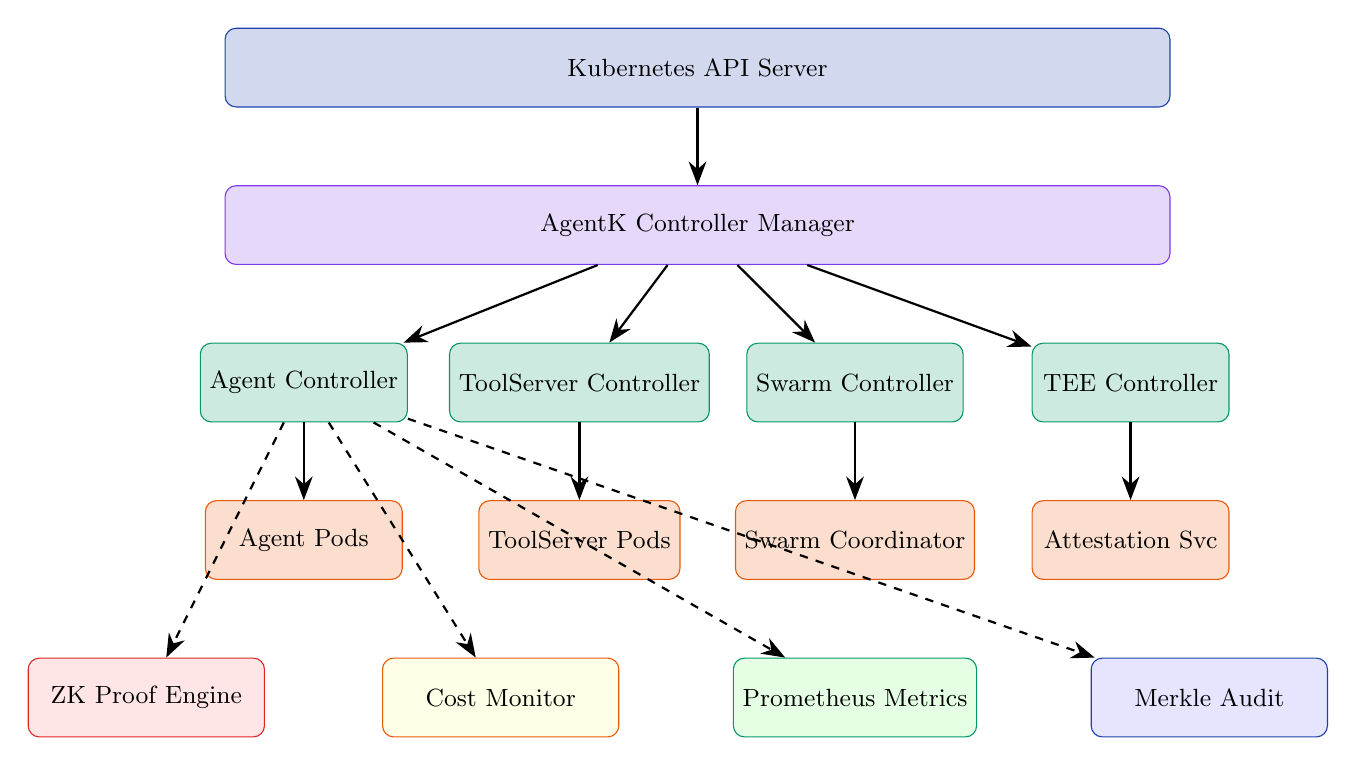
\begin{tikzpicture}[
    box/.style={rectangle, draw, rounded corners, minimum width=3cm, minimum height=1cm, text centered, font=\small},
    bluebox/.style={box, fill=agentk-blue!20, draw=agentk-blue},
    greenbox/.style={box, fill=agentk-green!20, draw=agentk-green},
    purplebox/.style={box, fill=agentk-purple!20, draw=agentk-purple},
    orangebox/.style={box, fill=agentk-orange!20, draw=agentk-orange},
    arrow/.style={-{Stealth[length=3mm]}, thick}
]

% Kubernetes API Server
\node[bluebox, minimum width=12cm] (api) at (0,6) {Kubernetes API Server};

% Operator
\node[purplebox, minimum width=12cm] (operator) at (0,4) {AgentK Controller Manager};

% Controllers row
\node[greenbox, minimum width=2.5cm] (ac) at (-5,2) {Agent Controller};
\node[greenbox, minimum width=2.5cm] (tc) at (-1.5,2) {ToolServer Controller};
\node[greenbox, minimum width=2.5cm] (sc) at (2,2) {Swarm Controller};
\node[greenbox, minimum width=2.5cm] (cc) at (5.5,2) {TEE Controller};

% Resources row
\node[orangebox, minimum width=2.5cm] (agent) at (-5,0) {Agent Pods};
\node[orangebox, minimum width=2.5cm] (tools) at (-1.5,0) {ToolServer Pods};
\node[orangebox, minimum width=2.5cm] (swarm) at (2,0) {Swarm Coordinator};
\node[orangebox, minimum width=2.5cm] (tee) at (5.5,0) {Attestation Svc};

% Arrows
\draw[arrow] (api) -- (operator);
\draw[arrow] (operator) -- (ac);
\draw[arrow] (operator) -- (tc);
\draw[arrow] (operator) -- (sc);
\draw[arrow] (operator) -- (cc);
\draw[arrow] (ac) -- (agent);
\draw[arrow] (tc) -- (tools);
\draw[arrow] (sc) -- (swarm);
\draw[arrow] (cc) -- (tee);

% Side modules
\node[box, fill=red!10, draw=agentk-red, minimum width=3cm] (zk) at (-7,-2) {ZK Proof Engine};
\node[box, fill=yellow!10, draw=agentk-orange, minimum width=3cm] (cost) at (-2.5,-2) {Cost Monitor};
\node[box, fill=green!10, draw=agentk-green, minimum width=3cm] (metrics) at (2,-2) {Prometheus Metrics};
\node[box, fill=blue!10, draw=agentk-blue, minimum width=3cm] (merkle) at (6.5,-2) {Merkle Audit};

\draw[arrow, dashed] (ac) -- (zk);
\draw[arrow, dashed] (ac) -- (cost);
\draw[arrow, dashed] (ac) -- (metrics);
\draw[arrow, dashed] (ac) -- (merkle);

\end{tikzpicture}
\end{center}

\section{Project Structure}

\begin{lstlisting}[style=bash, caption={Project directory tree}]
agentk-runtime/
+-- api/v1alpha1/           # 17 CRD type definitions (Go structs)
+-- cmd/
|   +-- main.go             # Operator entry point
|   +-- attestation-service/ # TEE attestation microservice
+-- config/
|   +-- crd/bases/          # Generated CRD YAML (13 files)
|   +-- manager/            # Operator deployment manifests
|   +-- edge/               # k3s/edge overlay (64Mi)
|   +-- attestation-service/ # TEE service deployment
+-- internal/
|   +-- controller/         # 30 files: reconcilers + helpers
|   +-- verifiable/         # ZK proofs (gnark circuits)
|   +-- tee/                # TEE attestation
|   +-- costintelligence/   # Real-time cost monitor
|   +-- costpredictor/      # Cost forecasting
|   +-- ebpf/               # eBPF policy generation
|   +-- governance/         # Autonomy levels 1-5
|   +-- lifecycle/          # Canary/rolling/blue-green
|   +-- merkle/             # SHA-256 Merkle tree
|   +-- observability/      # 30+ Prometheus metrics
|   +-- swarm/              # Multi-agent coordinator
|   +-- wasm/               # WasmEdge sandbox
|   +-- webhook/            # Admission webhooks
+-- web-dashboard/
|   +-- backend/            # FastAPI (Python)
|   +-- frontend/           # React/Vite/Tailwind
|   +-- Dockerfile          # Single-container build
+-- examples/               # 21 ready-to-use YAML samples
+-- docs/                   # AsciiDoc documentation (Antora)
+-- test/e2e/               # End-to-end tests
+-- benchmarks/             # Performance benchmarks
\end{lstlisting}

\section{Reconciliation Loop}

The heart of any Kubernetes operator is the \textbf{reconciliation loop}:

\begin{enumerate}
    \item User creates/updates an Agent resource (YAML)
    \item Kubernetes API server stores it in etcd
    \item AgentK controller receives a \texttt{Reconcile()} call
    \item Controller reads the current state (what exists) and desired state (what the YAML says)
    \item Controller creates/updates/deletes resources to match the desired state
    \item Controller updates the Agent's status with the current state
    \item If anything changes, the loop runs again
\end{enumerate}

\begin{keyconceptbox}
\textbf{Declarative vs Imperative}

Instead of saying ``create a deployment, then create a service, then set up health checks'' (imperative), you just say ``I want an agent with these specs'' (declarative) and the reconciler figures out what to do. If the deployment crashes, the reconciler automatically recreates it. This is why Kubernetes operators are so powerful.
\end{keyconceptbox}


% ============================================================================
% CHAPTER 22: CONTROLLER FLOWS
% ============================================================================
\chapter{Controller Flows}

\section{Agent Reconciler Flow}

When you create an Agent resource, here's what happens step by step:

\begin{enumerate}
    \item \textbf{Webhook validation}: The admission webhook checks if the YAML is valid
    \begin{itemize}
        \item Framework must be: google-adk, msaf, or custom
        \item Protocol type must be: A2A
        \item Replicas must be $\geq$ 0
        \item Port must be valid (1--65535)
    \end{itemize}

    \item \textbf{Reconciler starts}: \texttt{agent\_reconciler.go} is called

    \item \textbf{Build Deployment}:
    \begin{itemize}
        \item Select container image (template or custom)
        \item Configure environment variables (env + envFrom)
        \item Set resource limits (CPU/memory)
        \item Add volumes if specified
        \item Add readiness probe:
        \begin{itemize}
            \item A2A protocol: HTTP GET probe
            \item OpenAI protocol: TCP socket probe
        \end{itemize}
    \end{itemize}

    \item \textbf{Build Service}: Create a Kubernetes Service for network access

    \item \textbf{Apply ZK Proofs} (if \texttt{verifiable.proofMode} is set):
    \begin{itemize}
        \item \texttt{merkle-only}: SHA-256 hash chain checkpoint
        \item \texttt{snark-groth16}: Generate Groth16 proof via gnark
        \item \texttt{plonk-universal}: Generate PlonK proof via gnark
    \end{itemize}

    \item \textbf{Cost Intelligence} (if \texttt{costBudget} is set):
    \begin{itemize}
        \item Read from CostMonitor cache
        \item Apply action: none, downgrade, pause, or suspend
    \end{itemize}

    \item \textbf{Merkle Checkpoint}: Hash the current state into the audit trail

    \item \textbf{Update Status}: Write status fields (ready, serviceUrl, proofRoot, etc.)

    \item \textbf{Record Metrics}: Update Prometheus counters/gauges
\end{enumerate}

\section{ConfidentialAgent Reconciler Flow}

\begin{enumerate}
    \item Build the base Agent spec with TEE configuration
    \item Add attestation sidecar container
    \item Set security context (drop ALL capabilities, read-only filesystem)
    \item Add TEE-specific pod annotations
    \item Call attestation service with random nonce
    \item Verify ECDSA signature on the response
    \item Set \texttt{Verified = true/false} based on verification result
    \item If verification fails: requeue after 30 seconds
\end{enumerate}


% ============================================================================
% CHAPTER 23: DEPLOYMENT GUIDE
% ============================================================================
\chapter{Deployment Guide}

\section{Prerequisites}

\begin{itemize}
    \item Kubernetes cluster (v1.28+): Kind, GKE, EKS, AKS, or k3s
    \item kubectl configured to access the cluster
    \item cert-manager installed (for webhook TLS certificates)
\end{itemize}

\section{Step 1: Install cert-manager}

\begin{lstlisting}[style=bash, caption={Install cert-manager}]
kubectl apply -f https://github.com/cert-manager/cert-manager/\
releases/download/v1.19.1/cert-manager.yaml

kubectl wait --for=condition=ready pod \
  -l app.kubernetes.io/name=cert-manager \
  -n cert-manager --timeout=60s
\end{lstlisting}

\section{Step 2: Install the Operator}

\begin{lstlisting}[style=bash, caption={Install AgentK operator}]
kubectl apply -f https://github.com/agentic-layer/\
agent-runtime-operator/releases/download/v0.4.4/install.yaml

kubectl wait --for=condition=Available --timeout=60s \
  -n agent-runtime-operator-system \
  deployment/agent-runtime-operator-controller-manager
\end{lstlisting}

\section{Step 3: Deploy Your First Agent}

\begin{lstlisting}[style=bash, caption={Deploy a simple agent}]
cat <<EOF | kubectl apply -f -
apiVersion: runtime.agentic-layer.ai/v1alpha1
kind: Agent
metadata:
  name: my-first-agent
spec:
  framework: google-adk
  description: "A helpful AI assistant"
  instruction: "You are a helpful assistant."
  model: "gemini/gemini-2.5-flash"
  protocols:
    - type: A2A
  replicas: 1
  env:
    - name: GEMINI_API_KEY
      value: "your-key-here"
EOF
\end{lstlisting}

\section{Step 4: Verify}

\begin{lstlisting}[style=bash, caption={Verify the deployment}]
kubectl get agent my-first-agent
kubectl get deployment my-first-agent
kubectl get service my-first-agent
kubectl logs -l app=my-first-agent
\end{lstlisting}

\section{Edge Deployment (k3s)}

For resource-constrained environments:

\begin{lstlisting}[style=bash, caption={Deploy with edge profile}]
# Apply with edge overlay
kubectl apply -k config/edge/
\end{lstlisting}

This reduces operator memory from 128Mi to \textbf{64Mi} and CPU from 100m to \textbf{50m}.

\section{Flux GitOps Installation}

\begin{lstlisting}[style=yaml, caption={Flux OCI installation}]
apiVersion: source.toolkit.fluxcd.io/v1
kind: OCIRepository
metadata:
  name: agent-runtime-operator
  namespace: flux-system
spec:
  interval: 5m
  url: oci://ghcr.io/agentic-layer/manifests/agent-runtime-operator
  ref:
    semver: ">= 0, < 1"
---
apiVersion: kustomize.toolkit.fluxcd.io/v1
kind: Kustomization
metadata:
  name: agent-runtime-operator
  namespace: flux-system
spec:
  sourceRef:
    kind: OCIRepository
    name: agent-runtime-operator
  interval: 10m
  path: ./default
  prune: true
  wait: true
\end{lstlisting}


% ============================================================================
% CHAPTER 24: CODE WALKTHROUGH
% ============================================================================
\chapter{Code Walkthrough — Agent Creation End-to-End}

\section{The Complete Flow}

Let's trace what happens when you run \texttt{kubectl apply -f agent.yaml}:

\subsection{Step 1: YAML Submission}

Your YAML is sent to the Kubernetes API server. The API server checks:
\begin{itemize}
    \item Is the YAML valid against the CRD schema?
    \item Does the user have RBAC permissions to create Agents?
\end{itemize}

\subsection{Step 2: Webhook Validation}

Before storing the Agent, Kubernetes calls AgentK's \textbf{admission webhook} (\texttt{internal/webhook/v1alpha1/agent\_webhook.go}):

\begin{itemize}
    \item \textbf{Mutation}: Sets default values (framework, port, path)
    \item \textbf{Validation}: Checks field constraints (valid protocol, valid framework, valid port range)
\end{itemize}

\subsection{Step 3: Storage in etcd}

If the webhook approves, the Agent is stored in Kubernetes' database (etcd). This triggers a watch event.

\subsection{Step 4: Reconciler Activation}

The Agent controller (\texttt{internal/controller/agent\_reconciler.go}) receives the event and starts reconciliation:

\begin{lstlisting}[style=golang, caption={Simplified reconciler flow}]
func (r *AgentReconciler) Reconcile(ctx context.Context,
    req ctrl.Request) (ctrl.Result, error) {

    // 1. Fetch the Agent resource
    agent := &runtimev1alpha1.Agent{}
    r.Get(ctx, req.NamespacedName, agent)

    // 2. Build Deployment
    deployment := r.buildDeployment(agent)

    // 3. Build Service
    service := r.buildService(agent)

    // 4. Create or Update resources
    r.CreateOrUpdate(ctx, deployment)
    r.CreateOrUpdate(ctx, service)

    // 5. Generate ZK proof (if configured)
    if agent.Spec.Verifiable != nil {
        proof := r.ProofEngine.GenerateStepProof(...)
    }

    // 6. Check cost budget
    if agent.Spec.CostBudget != nil {
        decision := r.CostMonitor.GetDecision(...)
    }

    // 7. Update status
    agent.Status.ServiceUrl = serviceUrl
    r.Status().Update(ctx, agent)

    return ctrl.Result{}, nil
}
\end{lstlisting}

\subsection{Step 5: Kubernetes Takes Over}

Now Kubernetes:
\begin{enumerate}
    \item Schedules the Deployment's pods onto available nodes
    \item Pulls the container image
    \item Starts the container
    \item Runs the readiness probe
    \item Routes traffic through the Service
\end{enumerate}

\subsection{Step 6: Agent is Ready}

The agent is now running, accessible via its Service URL, and monitored by:
\begin{itemize}
    \item Kubernetes health checks (readiness/liveness probes)
    \item AgentK's cost monitor (checking budget every 60 seconds)
    \item AgentK's Merkle checkpointing (recording state at each reconciliation)
    \item Prometheus metrics (30+ counters and gauges being updated)
\end{itemize}


% ############################################################################
% APPENDICES
% ############################################################################
\appendix

% ============================================================================
% APPENDIX A: CRD REFERENCE
% ============================================================================
\chapter{CRD YAML Reference}

\section{Full Agent Spec}

\begin{lstlisting}[style=yaml, caption={Complete Agent spec with all fields}]
apiVersion: runtime.agentic-layer.ai/v1alpha1
kind: Agent
metadata:
  name: full-featured-agent
spec:
  # Core
  framework: google-adk      # google-adk | msaf | custom
  image: ""                   # Custom container image
  description: "My agent"
  instruction: "System prompt"
  model: "gemini/gemini-2.5-flash"
  replicas: 2

  # Communication
  protocols:
    - type: A2A
      port: 8000
      path: "/"

  # Tools & Sub-agents
  tools:
    - name: my_tool
      toolServerRef:
        name: my-toolserver
      propagatedHeaders:
        - Authorization
  subAgents:
    - name: helper
      url: "https://helper-agent.example.com"
      interactionType: tool_call

  # Security
  verifiable:
    proofMode: snark-groth16
  policyRefs:
    - name: network-policy
  toolSandboxRef:
    name: secure-sandbox

  # Cost
  costBudget:
    maxMonthlyCostUSD: "50.00"
    costPerTokenUSD: "0.00001"
    downgradeModel: "gemini/gemini-2-flash-lite"
  costIntelligence:
    optimizationMode: auto
    spotInstanceFallback: true
    suspendOnBudgetExhaust: true
    samplingIntervalSeconds: 60

  # Governance
  governance:
    autonomyLevel: 3
    requirePolicyCompliance: true

  # Lifecycle
  lifecycle:
    strategy: canary
    promptVersion: "v2"
    checkpointOnUpdate: true
    gracefulShutdownSeconds: 30
    selfHealing: true

  # Environment
  env:
    - name: API_KEY
      value: "secret"
  resources:
    requests:
      memory: "256Mi"
      cpu: "250m"
    limits:
      memory: "512Mi"
      cpu: "500m"
\end{lstlisting}


% ============================================================================
% APPENDIX B: PROMETHEUS METRICS
% ============================================================================
\chapter{Prometheus Metrics Reference}

All metrics are registered at the \texttt{/metrics} endpoint of the operator pod. They use the prefix \texttt{agentk\_}.

\section{Agent Reconciliation}

\begin{longtable}{p{6cm}p{2cm}p{5cm}}
\toprule
\textbf{Metric} & \textbf{Type} & \textbf{Labels} \\
\midrule
agentk\_agent\_reconcile\_total & Counter & name, namespace, result \\
agentk\_agent\_reconcile\_duration\_seconds & Histogram & name, namespace \\
agentk\_agent\_ready & Gauge & name, namespace, framework \\
\bottomrule
\end{longtable}

\section{Cost \& Tokens}

\begin{longtable}{p{6cm}p{2cm}p{5cm}}
\toprule
\textbf{Metric} & \textbf{Type} & \textbf{Labels} \\
\midrule
agentk\_tokens\_used\_total & Gauge & name, namespace \\
agentk\_predicted\_monthly\_cost\_usd & Gauge & name, namespace \\
agentk\_cost\_action\_total & Counter & name, namespace, action \\
agentk\_cost\_optimization\_actions\_total & Counter & name, namespace, mode \\
agentk\_spot\_instance\_enabled & Gauge & name, namespace \\
\bottomrule
\end{longtable}

\section{Policy, WASM, Merkle, Swarm}

\begin{longtable}{p{6cm}p{2cm}p{5cm}}
\toprule
\textbf{Metric} & \textbf{Type} & \textbf{Labels} \\
\midrule
agentk\_policy\_violations\_total & Counter & policy, namespace, rule, action \\
agentk\_policy\_reconcile\_total & Counter & name, namespace, type, result \\
agentk\_policy\_enforced & Gauge & name, namespace, type \\
agentk\_wasm\_sandbox\_ready & Gauge & name, namespace, runtime \\
agentk\_wasm\_sandbox\_reconcile\_total & Counter & name, namespace, result \\
agentk\_merkle\_checkpoint\_total & Counter & name, namespace \\
agentk\_merkle\_checkpoint\_count & Gauge & name, namespace \\
agentk\_swarm\_ready\_agents & Gauge & name, namespace, strategy \\
agentk\_swarm\_total\_agents & Gauge & name, namespace, strategy \\
agentk\_swarm\_reconcile\_total & Counter & name, namespace, strategy, result \\
\bottomrule
\end{longtable}

\section{Sovereign Features}

\begin{longtable}{p{6cm}p{2cm}p{5cm}}
\toprule
\textbf{Metric} & \textbf{Type} & \textbf{Labels} \\
\midrule
agentk\_simulation\_preview\_total & Counter & name, namespace, result \\
agentk\_zk\_proof\_chain\_length & Gauge & name, namespace \\
agentk\_attestation\_total & Counter & name, namespace, proof\_mode \\
agentk\_governance\_compliant & Gauge & name, namespace \\
agentk\_governance\_autonomy\_level & Gauge & name, namespace \\
agentk\_tee\_agent\_ready & Gauge & name, namespace, tee\_provider \\
agentk\_tee\_attestation\_total & Counter & name, namespace, tee\_provider \\
agentk\_workforce\_transitive\_agents & Gauge & name, namespace \\
agentk\_workforce\_transitive\_tools & Gauge & name, namespace \\
\bottomrule
\end{longtable}


% ============================================================================
% APPENDIX C: GLOSSARY
% ============================================================================
\chapter{Glossary}

\begin{longtable}{p{4cm}p{10cm}}
\toprule
\textbf{Term} & \textbf{Definition} \\
\midrule
\endhead
\textbf{A2A} & Agent-to-Agent protocol for inter-agent communication \\
\textbf{BN254} & Barreto-Naehrig 254-bit elliptic curve used in ZK proofs \\
\textbf{CRD} & Custom Resource Definition — extends Kubernetes with new resource types \\
\textbf{eBPF} & Extended Berkeley Packet Filter — kernel-level programmability \\
\textbf{ECDSA} & Elliptic Curve Digital Signature Algorithm \\
\textbf{etcd} & Distributed key-value store used by Kubernetes \\
\textbf{gnark} & Go library for zero-knowledge proof circuits (by Consensys) \\
\textbf{Groth16} & A zk-SNARK proof system with small proofs ($\sim$128 bytes) \\
\textbf{KZG} & Kate-Zaverucha-Goldberg polynomial commitment scheme \\
\textbf{MCP} & Model Context Protocol — standard for AI tool integration \\
\textbf{Merkle Tree} & Hash-based data structure for tamper detection \\
\textbf{MiMC} & ZK-friendly hash function (Minimal Multiplicative Complexity) \\
\textbf{OPA} & Open Policy Agent — policy engine using Rego language \\
\textbf{PlonK} & Universal SNARK system — no per-circuit trusted setup \\
\textbf{R1CS} & Rank-1 Constraint System — arithmetic circuit representation \\
\textbf{Reconciler} & Kubernetes controller loop that ensures desired state matches actual state \\
\textbf{SRS} & Structured Reference String — public parameters for PlonK \\
\textbf{TEE} & Trusted Execution Environment — hardware-sealed computing \\
\textbf{TDX} & Trust Domain Extensions — Intel's TEE technology \\
\textbf{SEV-SNP} & Secure Encrypted Virtualization — AMD's TEE technology \\
\textbf{WASM} & WebAssembly — portable binary format for sandboxed execution \\
\textbf{WasmEdge} & Lightweight WebAssembly runtime \\
\textbf{ZK-SNARK} & Zero-Knowledge Succinct Non-Interactive Argument of Knowledge \\
\bottomrule
\caption{Glossary of terms}
\end{longtable}

\end{document}
